\subsection{Opgave 31}

På figuren ses grafen for den lineære funktion f.

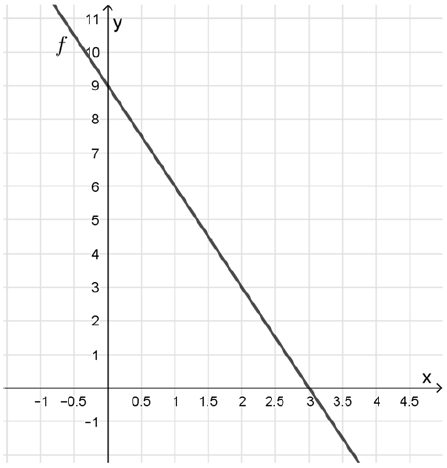
\includegraphics[width=8cm]{Opgave_31-40/Opgave_31/31.png}

a) Benyt figuren til at bestemme f(0)

\ans

For at finde $f(0)$ skal vi altså finde den y værdi vores funktion f har når 
vi står ved x værdien $x = 0$. Aflæser vi y værdien får vi at $f(0) = 9$.
Dette kan ses på figuren nedenfor

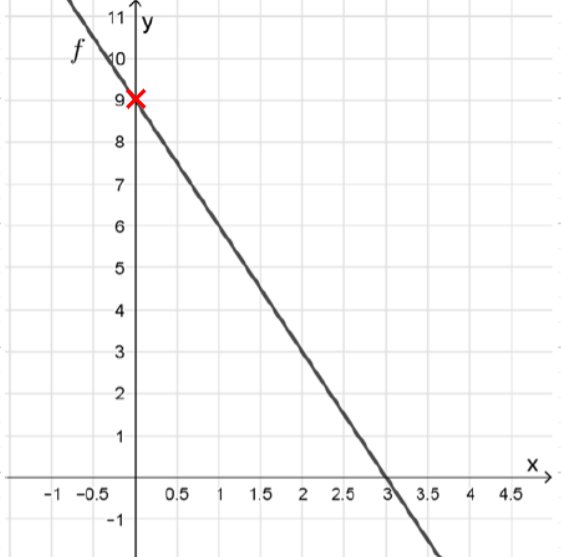
\includegraphics[width=8cm]{Opgave_31-40/Opgave_31/31.1.png}


b) Benyt figuren til at løse lignignen $f(x) = 0$

\ans

For at løse ligningen $f(x) = 0$ bliver vi bedt om at finde x værdien til funktionen f 
der hvor funktionen har y værdien 0 som er der hvor funktionen skærer x aksen.
Vi aflæser løsningen til $x = 3$.
Dette kan ses på figuren nedenfor

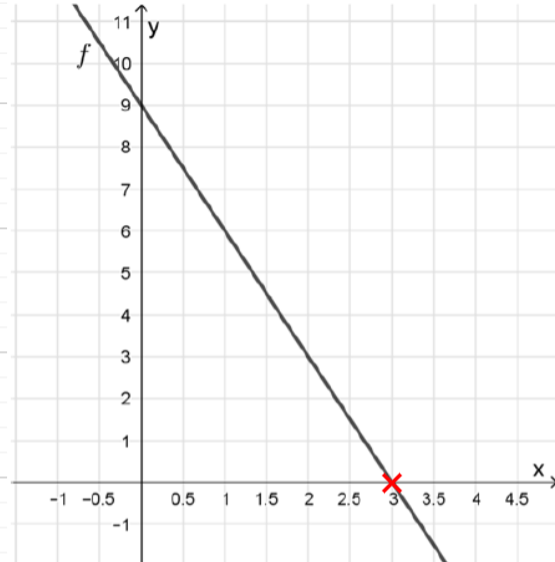
\includegraphics[width=8cm]{Opgave_31-40/Opgave_31/31.2.png}